\documentclass{../../myassignment}

\courselabel{IN1030}
\exercisesheet{Oblig 3}{Lover og etikk}

\usepackage{enumitem}

\usepackage{xcolor}
\definecolor{block-gray}{gray}{0.85}
\usepackage{environ}
\NewEnviron{myblock}
{\colorbox{block-gray}{%
\parbox{\linewidth\relax}{%
\small\addtolength{\leftskip}{-5mm}
\addtolength{\rightskip}{0mm}
\BODY}}
}
\renewcommand{\quote}{\myblock}
\renewcommand{\endquote}{\endmyblock}

\begin{document}

\section*{Oppgave 1 --- Universell utforming}
	\begin{problem}
		Se videoen \textit{Ein introduksjon til universell utforming} som du finner her: \url{https://uu.difi.no/krav-og-regelverk/losningsforslag-web/film-med-24-tips}. Velg ut tre av de 24 tipsene som presenteres i videoen, og forklar disse tre. Bruk gjerne eksempler for å illustrere hvordan disse kan implementeres i praksis.
	\end{problem}
	\begin{answer}
		\begin{description}[style=nextline]
			\item [Bruk riktig kode og strukturer teksten]
				WYSIWYM --- Ved å skrive hva vi mener, syntax-vis, i steden for hvordan vi ønsker at det skal se ut, siden innhold er viktigere enn utseende, kan vi la brukeren, eller navigatøren hen bruker, selv velge hvordan ting skal presenteres for brukeren. For eksempel kan vi se dette i HTML, der vi har objekter (altså tags) med klasser og id'er. Vi bruker klasser til å definere hva innholdet i taggen skal inneholde, og vi kan gjerne bruke CSS for å definere hvordan hvert type objekt skal plasseres og sees ut på siden vår.

				Bootstrap, som er en kjent og velbrukt framework for HTML+CSS, sliter med akkuratt dette, siden vi ikke definerer hva objektene representerer, men heller hvordan vi ønsker at det skal bli vist. Ved å bruke denne metoden, som kan på et vis ligne på WYSIWYG, mister brukeren og andre utviklere muligheten til å lett referer til alle objekter av samme type, og dermed vanskeliggjør tilgjengligheten av nettsiden.

			\item [La alt innhold nås med tastatur]
				Jeg bruker selv nesten aldri mus. Jeg har ikke tre hender. Jeg synes det er slitsomt å holde på musen i flere timer, siden disse ikke alltid er like ergonomiske. I tillegg må jeg sikte, og det er ikke alltid jeg finner musen på skjermen siden den er så liten. Det er stort sett mye lettere å tabulere seg fram til det en ønsker, så lenge det ikke er mange objekter i programmet, og programmet viser hva vi ``peker'' på. 

				Jeg programmerer stort sett i Vim for samme grunnen. Jeg kan si til programmet nøyaktig hva jeg ønsker å gjøre, i steden for å måtte gjøre det selv. Det gjør arbeidet mye lettere, siden jeg ikke trenger å tenke på hvordan programmet jeg bruker forventer at jeg skal gjøre det. Så lenge et program er vel-dokumentert er det stort sett lettere å skrive kommandoer/utrykk enn å navigere rundt i menyer for å lete etter ting. Alle kan jo engelsk, men UI/UX er forvirrende.

				X server was a mistake. 

			\item [Tekst video]
				Alle burde ha rett til å kunne se videoer, filmer, og lignende. Hvis ikke vi legger til undertekst eller transcriptions av det som blir sagt pá videone mister døve personer, eller personer med nedsatt hørselsevne muligheten til å ha tilgang til samme innholdet personer uten sensorielle funskjonshemmelser. Til og med folk som i grunnen er ``i grei tilstand'' vil ha nytte av dette, siden man ofte kan lese ting raskere enn det videon presenterer informasjonen på; dialekten er litt ukjent, og man ikke får med seg alle ordene, eller det er visse ord som er ukjente siden de hører til et felt man ikke kjenner til. Det finnes sikkert mange andre fordeler med å ha undertekst, uten at de er nevnt her.

		\end{description}
	\end{answer}


	\begin{problem}
		Forklar med egne ord de fire WCAG 2.0 prinsippene. Velg deretter ut og beskriv én retningslinje for hver av de fire prinsippene. Bruk eksempler for å illustrere hvordan dette kan brukes i praksis. Den norske oversettelsen av WCAG 2.0 finner du her: \url{https://www.w3.org/Translations/WCAG20-no-20110926/}
	\end{problem}
	\begin{answer}
		\begin{description}[style=nextline]
			\item [Persepsjon] Alle skal ha muligheten til å oppfate innholdet som er på siden, uavhengig av platform, funskjonsnedsettelser, eller andre variabler. Et eksempel på dette kan være fargeblindhet: vi må ikke bruker farger oppå hverandre som gjør at enkelte personer mister muligheten til å lese teksten. Store kontrastnivåer gjør susen.
			\item [Operasjon] Alle, uavhengig av input-type, må ha muligheten til å bruke nettsiden eller applikasjonen. Noen bruker tastatur, noen bruker touch-skjerm, mens andre kun bruker tale, som eksempler. Man må lage løsninger for alle grensesnitt, slik at ingen blir utelukket. 
			\item [Forståelig] Innholdet i siden må ikke være vanskelig å tolkes. Dette inkluderer hvordan vi setter opp menyer, hvor vi plasserer tekst i forhold til bilder, og alt annet innhold på nettsiden. Poenget er at personer meg kognitive vanskeligheter ikke skal føle seg truet av nettsiden, og lett kan bruke applikasjonen på lik linje med alle andre. 
			\item [Robust] Det siste prinsippet sier at innholdet på siden må være satt opp på en måte som gjør at enhver teknologi, uavhengig av hvordan de implementerer standarer, har muligheten til å tolke, lese og gjenskape innholdet vi presenterer. Med andre ord betyr dette at text-to-speech services må fungerer på kryss og tvers av platformer, nettlesere, og annet brukerspesifikt utstyr, som et eksempel. 
		\end{description}
		Ved å bruke standarerer og velkjente APIer kan de fleste problemerer som eventuelt oppstår i visse situasjoner bli utelukkede, siden et abstraksjonsnivå som er velbrukt av mange protokoller og tjenester vil være ganske polert over tid. I tillegg er slike frameworks ofte sertifiserte, slik at vi kan garantere en viss WCAG-kvalitet. Hvis vi gjør ting manuelt må vi passe på å gå gjennom alle reglene, og teste for alle situasjoner selv. Dette kan fort bli vanskelig om applikasjonen ikke har en standard-form eller er av en ``plain og kjedelig'' faktor.
		
	\end{answer}

	\begin{problem}
		Beskriv en av endringene som er gjort fra WCAG 2.0 til WCAG 2.1
	\end{problem}

	\begin{answer}
		Man må nå ha mulighet til å kansellere en handling etter at man har klikket mouse-down, enten ved å dra musa vekk fra knappen, eller på andre måter. I syvende og sist kan ikke mouse-down bli brukt til å utføre endelige funskjoner. 
		
	\end{answer}

	\newpage

	\begin{problem}
		Beskriv disse begrepene (minimum én setning for hvert begrep):
	\end{problem}
	\begin{answer}
		\begin{description}[style=nextline]
			\item [Universell utforming]  Universell utforming er et generisk begrep som inkluderer en del prinsipper som gjør at folk med bevegelsehindringer kan leve opp til den retten de har, på samme måte som folk uten handicap gjør det. I praksis betyr dette at selve arkitekturen til ei bygning er inkluderende, og at ikke det er særløsninger for rullestolbrukere i forhold til andre brukere.

			\item [Inkludering] Inkludering er et begrep som kan brukes i flere sammenhenger. Det kan referer til hvordan vi bruker språket, hvordan vi takler situasjoner angående mennesker (eller andre vesener med følelser), eller hvordan et sted ---i alle sine betydninger--- er tilrettelagt for forskjellige vesener.

			\begin{figure}[h]\begin{center}
					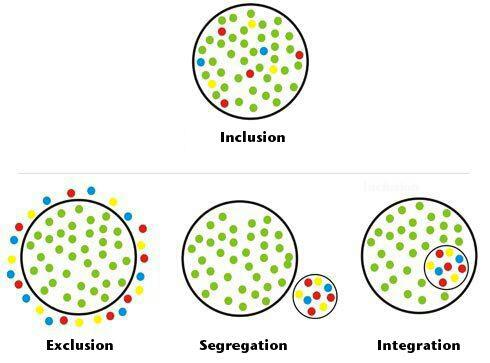
\includegraphics[scale=0.6]{inclusion.jpg}
					\caption{From \url{https://tex.stackexchange.com/questions/314319}}
			\end{center}\end{figure}

			\item [Tilgjengelighet] Konseptet for tilretteleggelsen av et generisk system for folk med handicaps, uførhet, eller andre vanskeligheter blir kalt for tilgjengelighet. Generelt sett blir jo ordet brukt for å se hvor ``tilgjengelig'' noe er, altså hvor lett det er å få tilgang til en informasjon, tjeneste, eller sted.

			\item [Sosial modell] Den sosiale modellen av funskjsonshemmelser er en måte å tolke og/eller forstå virkeligheten på, fra et filosofisk ståsted. Forskjellige modeller har foskjellige synsvinkler når det gjelder ``hva'' som er ``riktig'' angående funskjonsnedsettelser og samfunnet, og hva som er ``problemet''. 

			Den sosiale modellen sier, kort sagt, at problemet ikke ligger ved personene, men heller ved samfunnet. Det er samfunnets ansvar å tilrettelegge for at alle i samfunnet skal ha plass og mulighet. Hvis noen ikke har plass er det ikke dem som er ``syke'', ``feil'' eller ``gale'', men heller samfunnet som er ``laget'' på feil måte.

		\end{description}
	\end{answer}

	\newpage

	\begin{problem}
		I denne oppgaven blir du invitert til å reflektere over hva tilbakemelding betyr for deg med tanke på inkludering og universell utforming i enstudiesituasjon. Tenk deg tre ulike situasjoner for tilbakemeldinger.

		\begin{itemize}
			\item[---] Tilbakemelding ansikt til ansikt fra eller til medstudenter, gruppelærere eller foreleser
			\item[---] Tilbakemelding fra eller til medstudenter, gruppelærere eller foreleser via et digitaltsystem som e-post, Devilry, melding
			\item[---] Tilbakemelding fra eller til et digitalt system som bekreftelse på at en fil er lastet oppeller at du godtar at cookies blir lagret
		\end{itemize}
		Sammenlign minst to av situasjonene med tanke på universell utforming. Beskriv hva somgjør at du kan oppleve at du er inkludert eller ekskludert? Bruk gjerne konkrete eksempler.
	\end{problem}

	\begin{answer}
		Når det gjelder å inkludere folk som et samfunn, må vi vite og ha i bakhodet at det er forskjeller mellom individene. Alle er ikke like flinke til de samme tingene. Noen er flinkere med matematikk, mens andre er flinkere med presentasjonsteknikker. Å få tilbakemeldinger på obliger, altså hva brukeren har gjort/laget selv, lar brukeren se hva hen sliter med, og hva hen må fokusere mer på. Ikke bare vil hen vite hvor bra hen presterte på en prøve eller innlevering, men brukeren vil vite presist hva som ble gjort bra, dårlig, og eventuelt hva som kunne blitt gjort bedre. Nå vet brukeren det til neste gang. 

		Å gjøre obliger, i seg selv, er nyttig fordi at eleven kan reflektere selv over faget som hen studerer, allerede før eksamen. Frivillige obliger, eller treningsoppgaver kan jo teoretisk ha den same funskjonelle funskjonen; men det er ikke alle som er like flinke til å prestere uten et eksternt press. Eleven som sliter med faget vil bruke lenger tid på obligene, mens en annen elev som synes faget er nokså lett vil bli ferdig raskere med obligen. Eventuelt vil den andre eleven bruke den ekstra tiden på å utdype kunnskapene i det spesifike faget. Alle får slik en mulighet til å lære, og alle vil få svar på eventuelle spørsmål, og tilbakemelding på det de har jobbet med. 

		Som et siste punkt ønsker jeg å nevne at spill som Kahoot kan styrke læringsprosessen, selv om konkuranse-spill ofte har motsatt effekt: der vinnerene får et kick av å være best, mens ``taperene'' blir skuffet over egne resultater, og tror at de ikke har muligheten til å bli like flinke. I og med at Kahoot-spillene som blir gjort på skolen ikke har premier, og er generelt sett ganske ``snille'', og at vi i tillegg får umiddelbare svar fra læreren om spørsmålene ---noe som klarerer Frequently Asked Questions, og eventuelle misforståelser som kan ha kommet frem i timen--- tenker jeg at dette er en positiv måte å undervise på for alle. 

	\end{answer}

\newpage
\section*{Oppgave 2 --- Personopplysninger}
	\begin{problem}
		Les artikkelen om Folkeopplysningen og hvordan informasjonen Facebook lagrer om deg kan bli misbrukt. Se deretter Youtube-klippet om hvordan Cambridge analytics bruktepersonopplysninger. Lenker til artikkelen og dokumentaren finner du nedenfor. Beskriv dilemmaene som tas opp i artikkelen og Youtube-klippet. Skriv minimum ett avsnitt.
	\end{problem}

	\begin{answer}
		Å vite hvordan realiteten rundt oss fungerer var allerede et tema rundt Sokrates' og Plato's tid. Sofistene brukte sin kunnskap om retorikk og tale for å manipulere samfunnet slik de så virkeligheten. Dette var 2700 år siden, ish. 

		For å være frie mennesker har vi et krav på å kunnskap. Kunnskap om hvilken informasjon vi blir utsatt for, og mulighet til å kontrastere informasjon som vi blir vist til. Når dette blir gjort i våres underbevissthet, ved å endre på hva vi faktisk kan se, og dermed også hva vi tenker på mister vi muligheten til å te egne, frie og selvstendige valg. Vi mister menneskeligheten vår, og, som Kant ville sagt, blir vi ikke behandlet som rasjonelle vesener. Dette har vi en rett på, fra et etisk synspunkt.

	\end{answer}

	\begin{problem}
		Se for deg at du tar opp lyd eller tar bilde i en av gruppetimene dine. Er det nødvendig å informere de som er tilstede om opptaket og i så fall hvordan ville du gått fram?
	\end{problem}

	\begin{answer}
		I forhold til personvernsloven er det ikke lov å filme andres private eiendom, eller offentlige steder uten særtilatelse og godkjennelse av de som blir filmet. Selv ikke til privatbruk. Om man skal filme gruppetimene må alle som er tilstede i klasserommet forstå, og godkjenne, at timene blir filmet. Hvis gruppetimene hadde vært private, altså gjennomførte på et privat sted, ville det vært nok å informere om opptakene. 

	\end{answer}

	%\newpage

	\begin{problem}
		En IT-bedrift som behandler personopplysninger beslutter å legge lagring og behandling av personopplysninger til en skytjeneste lokalisert i utlandet. Er dette lov ifølge Personopplysningsloven? Husk å henvise til lovverket. Hva må bedriften gjøre for å kunne outsource lagring og behandling av personopplysninger?
	\end{problem}

	\begin{answer}
		Personopplysningsloven eksisterer for å beskytte personene sine dataer. Alle som faller under GDPR / Personopplysningslovens beskyttelse har rett til å være beskyttet mot hvem som helst andre. Det har ikke noe å si hvem som ønsker å bruke personopplysningene dine, siden de må følge GDPR sine krav. Til og med utenomjordiske vesener har ikke noe de skulle sagt. Artikkel 3.1 av GDPR og artikkel 3.2 definerer dette ganske tydelig. For å kunne outsource lagring og behandling av personopplysninger må bedriften få fullstendig samtykelse av alle personene de samler data av, i tillegg til at disse må kjenne til sine rettigheter angående personopplysninger.

		Dersom en IT-bedrift likevel ønsker pga. nødvendighet å lagre og behandle dataer i utlandet, må brukerene bli tydelig bli informert over risikoene som eventuelt kan forekomme av å være utenfor det beskyttede området. I en situasjon hvor en bindende avtale skaper et krav om at personopplysningene må bli behandlet i et internasjonalt sammenheng, må denne avtalen inkludere en del opplysninger som tilsvarer kravene til GDPR. Databehandleren vil ha ansvaret over eventuelle feil som kan skje, om ikke hen klarer å bevise uskyldighet. 

		Et untakk til det siste avsnittet finnes i visse land som er forhåndsgodkjente av GDPR-komisjonen, der disse territoriumene er vedtatte som sikre soner.

	\end{answer}

	\begin{problem}
		Finn frem til personvernerklæringen til det systemet du har jobbet med (NF-kino, Vy,Kolonial eller Yr). Hvem kan brukerens personopplysninger utleveres til? Det holder å nevne to interessenter/aktører i denne oppgaven. Hvis det er vanskelig å finne konkreteinteressenter/aktører kan du reflektere rundt hva dette har å si for brukeren.
	\end{problem}

	\begin{answer}
		Yrgruppen.no nevner kun ``tredjepartier'' og staten som interessenter. Tredjepartier kan jo bety alt fra Google Analytics, til Ruter. Jeg spurte derfor via chat-tilbudet de har, og fikk følgende respons: 

			\begin{quote}
				\begin{description}
					\item [09:50:02] Du er plassert i kø
					\item [09:50:40] Erik er nå tilkoblet
					\item [09:50:40 Erik] Hei og takk for at du tar kontakt med oss. Jeg heter Erik, hva kan jeg hjelpe deg med?
					\item [09:50:40 Mazunki] Hei. Jeg lurte på hvilke selskap dere deler personopplysninger med, siden den eneste informasjonen jeg finner er en ganske generisk ``tredjepartier'' og staten.
					\item [09:54:30 Erik] Deler info med andre togoperatører i Norge, men kun det som går på selve reisen/billetten, altså navn, tlf nr og e-post. Vi deler ikke andre personopplysninger.
					\item [09:57:42 Mazunki] Hva er grunnen til at tlf.nr og e-post blir delt med andre togoperatører? Jeg kan tenke meg at navn blir brukt som en form for identifikator for å se hvem som reiser hvor.
					\item [10:05:16 Erik] Det er for eks ved bekreftelse på reise eller for å søke opp en bestilling, hvis konduktør ikke finner en billett.
					\item [10:06:49 Mazunki] Ah, så informasjonen blir kun delt i en direkte handel-sammenheng, og ikke som en del av markedsføring eller datanalyse?
					\item [10:07:33 Erik] Nei, kun for reisesammenheng.
					\item [10:07:44 Mazunki] Kult, takk. :)
					\item [10:08:19 Mazunki] Kan jeg referere til denne samtalen i en skoleoppgave?
					\item [10:09:28 Erik] Ingen årsak. Skulle ikke være noe problem med det, for det er denne infoen jeg har fått fra skiftleder. Denne info blir kun delt i reisesammenheng mellom togoperatørene.
					\item [10:10:15 Mazunki] Supert! Ha en forsatt fin dag.
					\item [10:10:25 Erik] Det samme ønskes deg.
					\item [10:10:28] Chatten er avsluttet.
				\end{description}
			\end{quote}

	\end{answer}

\newpage

\section*{Oppgave 3 --- Digitalisering, automatisering, og etisk refleksivitet}
	\begin{problem}
		Se filmen om etiske dilemma ved programmering av førerløse biler av Patrick Lin (4:15min). Redegjør for dilemmaet som tas opp i denne videoen. Drøft mulige tilnærminger for åjobbe med dette dilemmaet. Skriv minimum ett avsnitt. Filmen finner du her: 

		\url{https://www.youtube.com/watch?v=ixIoDYVfKA0}
	\end{problem}

	\begin{answer}
		Det etiske dilemmaet som presenteres i videoen visualiserer problemet vi har angående å stole på datamaskiner, nokså rasjonelle ``ting'' til å ta valg for oss. Vi tenker at datamaskiner er enten dumme eller smarte, men det er ikke så rett fram i virkeligheten. Alt i alt vil et selvkjørende kjøretøy ha mye raskere reaksjonstid en det et menneske vil ha, og vil klare å regne ut det beste valget mye raskere en det vi selv klaerer. Foreløpelig har vi en naturlig evne til å reagere på ren intuisjon, som ikke maskiner ennå har, men likevel vil autonome biler redusere det totale antall ulykker drastisk over tid. 

		Det finnes ikke noe klart svar på hvordan vi kan tilnærme oss denne problemstillingen, annet en å vente til vi kan garantere null ulykker. Dette vil aldri skje, siden transisjonen mellom menneskestyrte kjøretøy og selvkjørende kjøretøy vil ha visse problemer i startfasen, siden folk ikke stoler på maskinene, og er ikke vant til hvordan det fungerer. Et helt system av maskinstyrte kjøretøy vil ha muligheten til å kunne kommunisere med hverandre med perfekt synkronisasjon takket være at de er maskiner som har interne klokker, noe som kan skape en flyt mennesker ikke er i stand til, rett og slett pga. en teknisk limitasjon. 

		Selv tenker jeg menneske-drevne, ikke-fornybare og private kjøretøy burde ulovlig-gjøres ummidelbart, men det er ikke like lett å få alle på samme side når det gjelder såpass drastiske endringer. La oss innovere både bedre teknologi, og skape en fullstendig transisjonsplan, for å så gjennomføre denne vis a vis staten. 
	\end{answer}

	\begin{problem}
		Hva menes med etisk refleksivitet?
	\end{problem}

	\begin{answer}
		Etisk refleksivitet er noe man må tenke på når man utvikler. Det handler om å analysere hva som kan gå rett og galt, hvilke risikoer som fremkommer med det vi arbeider med, og eventuelt hvordan resultatene kan forebygge eller foreverre samfunnet generelt. Det er viktig å tenke på dette i nesten alle sektorer, og dermed ha med en spesialist innenfor etikk, eller eventuelt konsultere med et selskap som gjør etiske valg.

		Et godt eksempel på dette er vist i videoen om Mehdi Ettehadulhagh. Det ble gjort en etisk beslutning angående deltakeren med tanke på eventuelle traumaer som kan fremstå i å sette personen i den situasjonen. Dette blir ofte gjort i ``Trolley dilemma''-eksperimenter også, der ``skuespillerene'' kan få panikk og traumaer av å ta ``feil'' valg. Disse er eksemplere på ganske direkte etiske valg, mens ofte kan refleksiviteten komme fra helt andre retninger. 

		Noen godt råd er å spørre seg selv: ``Er det jeg gjør nå noe som er positivt, bra, og riktig for resten av sammfunnet? Ville jeg likt å bli behandlet slik? Kommer det til å komme mer nytte enn skade av de valgene jeg tar?'' Mitt svar til disse spørsmålene er at jeg ikke vet, stort sett. Jeg kan anta hva som er universelt riktig, og så lenge jeg prøver å finne ut av hva som er best så er jeg hvertfall på riktig spor. 
	\end{answer}

\newpage

\section*{Oppgave 4 --- Spørsmål til pensumartikkelen}
	\begin{problem}
		Les artikkelen Five provocations for ethical HCI research som ligger underpensum/læringskrav. Skriv to spørsmål til  ettav de fem dilemmaene. Det kan være noe dulurer på, er usikker på, eller gjerne vil vite mer om. HCI står for Human Computer Interaction.
	\end{problem}
	\begin{answer}
		\begin{itemize}
			\item [---] You refer to the right to be anyonmous in research papers. Are there any relevant cases where the subjects themselves actually matter for the sake of knowledge? With this I mean: isn't it possible to present the same information without relating the topics to direct examples of the real world?
			\item [---] We're talking about ethics about people. We want to respect the anonymity of human beings. What about the anonymity of artificial computers? Or non-human animals? Why are we only considering humans when we are considering the ethics of it all?
		\end{itemize}
	\end{answer}


\section*{Oppgave 5 --- Refleksjon}
	\begin{problem}
		Skriv noen setninger om hva du har lært gjennom å jobbe med denne obligen. Hva likte du? Var det noe som var tankevekkende?
	\end{problem}

	\begin{answer}
		Denne obligen har vært ganske ``spot on'' med tanke på hva jeg ønsker å spesialisere meg i. Jeg har vurdert, før denne obligen, å studere kognitiv filosofi, etikk, og samfunnsutvikling. Jeg vet ikke helt hvordan jeg kan gå videre etter jeg har studert filosofi+etikk, i tilleg til en bachelor i robotikk, med tidligere data-science i lomma... men jeg håper jeg kan gjøre en del research innenfor etikken og filosofien av utviklingen. Kanskje gjøre research på hva som gjør et menneske til et menneske, og en datamaskin med kunstig inteligens til en ``død gjenstand'' (om det er alt den er / kommer til å forbli for alltid...)

	\end{answer}



\end{document}